\documentclass[11pt]{article}
\usepackage[a4paper,margin=1.5cm,top=0.8cm]{geometry}
\usepackage{graphicx}
\usepackage[colorlinks=true,linkcolor=blue,urlcolor=blue,citecolor=blue]{hyperref}
\usepackage[backend=biber]{biblatex}
\addbibresource{coalescence.bib}
\title{Drop size distribution from the breakup rate}
\author{Ianto Cannon, \today}
\date{}
\begin{document}
\maketitle

We follow the model of \textcite{garrett00connection}, in which drops of diameter $d$ break into $m$ equally sized daughter drops. Volume conservation sets the daughter-drop diameter to $d' = d / m^{1/3}$. In steady state, the rate of drop removal equals the rate of creation,
\begin{equation}\label{eqGarrett}
N(d')\,\tau(d')\,d' = m\,N(d)\,\tau(d)\,d,
\end{equation}
where $\tau(d)$ is the drop lifetime before breakup, and $N(d)\Delta d$ is the number of drops with diameters in the range $d$ to $d+\Delta d$.

The classical inertial-range estimate for the breakup lifetime is the eddy turnover time,
\begin{equation}\label{eqCT}
\tau_d = \frac{d^{2/3}}{\epsilon^{1/3}},
\end{equation}
which applies when surface tension is negligible.

The model proposed by \textcite{coulaloglou77description} and measured by \textcite{vela-martin22memoryless} accounts for the suppression of breakup near the Hinze scale $d_H = 0.725\,\sigma^{3/5}\rho^{-3/5}\epsilon^{-2/5}$. This leads to an exponential breakup lifetime,
\begin{equation}
\tau_{CT} = \frac{d^{2/3}}{14.8\,\epsilon^{1/3}} \exp\!\left(\frac{-7.8\,\sigma}{\rho\,\epsilon^{2/3} d^{5/3}}\right).
\end{equation}

We start with a single drop of size $8d_H$, which lies in the inertial range, so that the subsequent cascade is insensitive to the precise initial size. At each step, equation~\ref{eqGarrett} gives $N(d')$ from the known $N(d)$, allowing us to iteratively solve toward smaller diameters using $\tau=\tau_d$ (empty circles) and $\tau=\tau_{CT}$ (filled circles). This procedure is analogous to injecting drops of size $8d_H$ at a constant rate and allowing them to breakup in a turbulent flow.

Both models converge to the inertial-range prediction
\begin{equation}
N(d) \sim (d/d_H)^{-10/3},
\end{equation}
because far above $d_H$ both lifetimes scale as $d^{2/3}$, so the steady state condition necessarily produces the classical $d^{-10/3}$ drop size distribution. Near $d_H$, however, the \textcite{coulaloglou77description} lifetime predicts thousands of times more drops because surface tension greatly prolongs the breakup time. In this analysis we choose binary breakups ($m=2$), but the resulting distributions are in fact insensitive to the choice of $m$ and to any overall prefactor in the breakup rate (such as the $14.8$ in equation~\ref{eqCT}). This invariance arises because $N(d')$ depends on the ratio $\tau(d)/\tau(d')$, causing such constants to cancel.
\begin{figure}[h!]
    \centering
    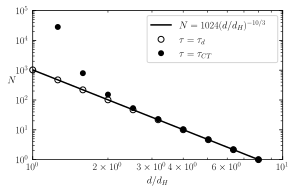
\includegraphics[width=.6\textwidth]{popBalance.pdf}
\end{figure}
\newpage
\printbibliography
\end{document}

